\chapter{\sysname{} Design}
\label{sec:system-design}

In this chapter, I present the design of \sysname{}. The primary goal of
\sysname{} is to enable applications with the ability to adapt its communication
while maximizing its utility.

\section{Challenges}
\label{sec:challenges}

\noindent There are four challenges in realizing \sysname{}.

\para{C1: Diverse application and data:} As discussed in~\autoref{sec:bat}, the
best adaptation scheme is often application- and context-specific
optimizations. It becomes important to separate individual application logic
from specific degradation strategy as well as the concrete mechanisms.

\para{C2: No analytical solutions:} Unlike SQL queries whose demand and accuracy
can typically be estimated using analytical models~\cite{cormode2012synopses},
many of our streaming applications are dealing with unstructure data using
either use blackbox operations (such as H.264 encoding) or non-linear operators
(such as thresholding). The effect of these degradations is not immediately
available.

\para{C3: Multi-dimensional exploration:} Real-world applications typically have
more than one tunable parameters; leading to a combinatorial space for
exploration. In addition, these parameters are not necessarily orthognal.  The
optimal degradation strategies may only be achievable when more than one
degradation is in effect.

\para{C4: Runtime adaptation at application layer:} Although recent work on
resource reservation makes it possible to guarantee quality of service with new
IP or MAC layer protocols in LAN (e.g. TSN~\cite{johas2013heterogeneous}), we
target at WAN analytics where most of the infrastructure is owned by others and
shared among many users. An application-layer solution is in favor to those that
require special hardware or software upgrade.

\section{System Architecture}
\label{sec:architecture}

\begin{figure*}
  \centering
  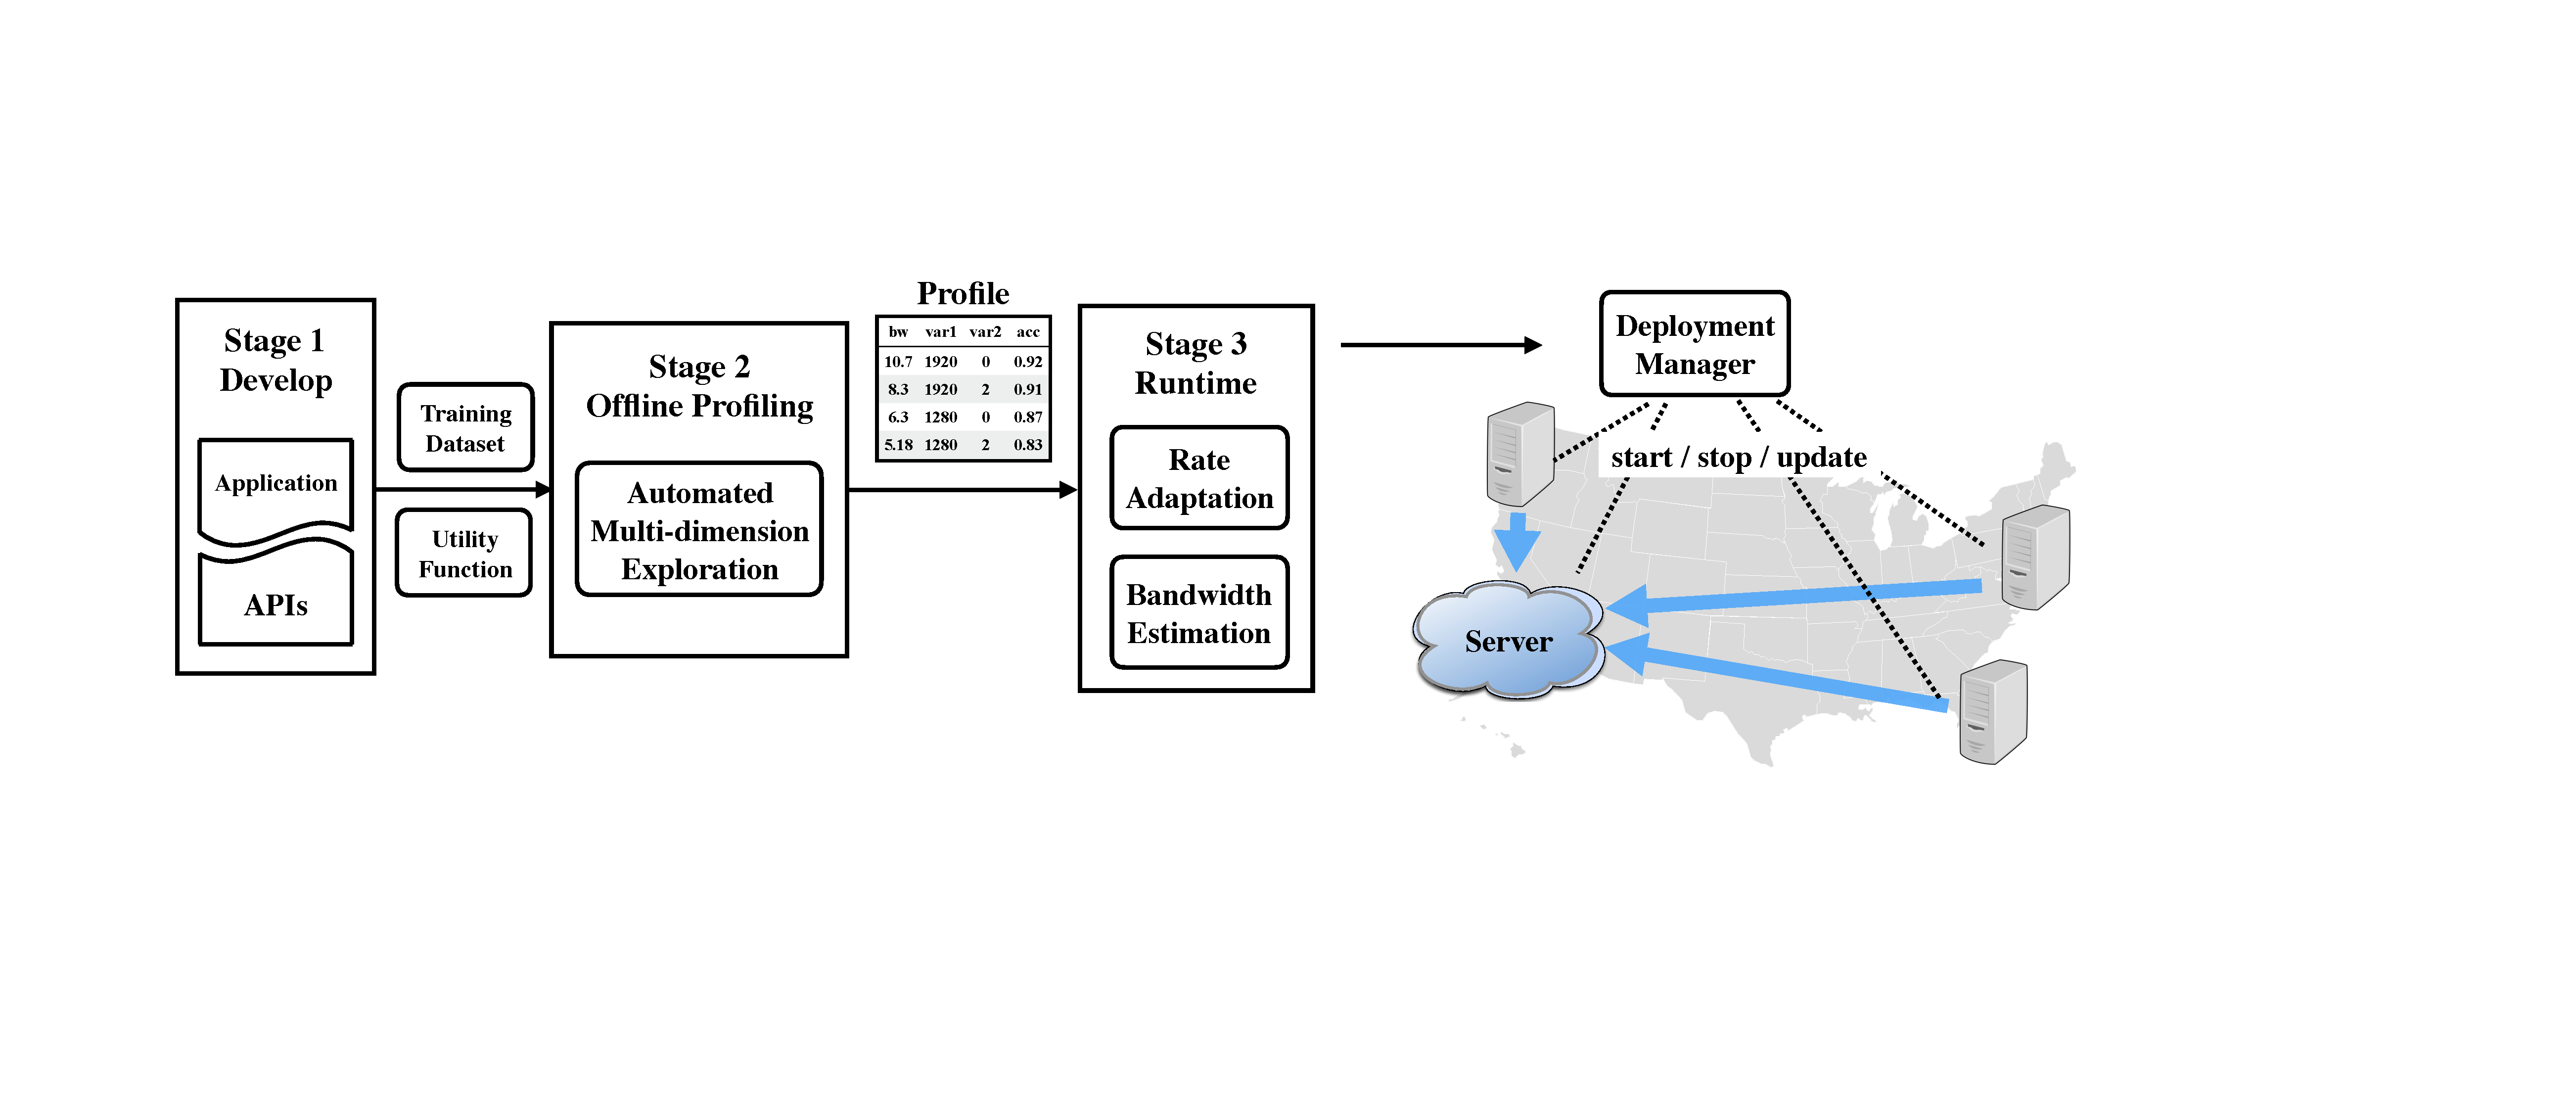
\includegraphics[width=\linewidth]{figures/arch.pdf}
  \caption{The three-stage architecture of \sysname{}.}
  \label{fig:overview}
\end{figure*}

To address the aforementioned challenges, \sysname{}'s solution is split into
three parts (\autoref{fig:overview} illustrates them).

\para{Programming abstraction~(\autoref{sec:prog-abs}):} Applications are
modelled as a directed acyclic graph (DAG) of computations. In addition to the
normal operators from existing systems, I propose a novel set of \texttt{maybe}
operators to express the specification of degradations. The proposed APIs do not
require developers to be exact on the quantity, making effort to integrate with
existing applications minimal.

\para{Automatic multi-dimensional profiling~(\autoref{sec:profiling}):} The
system automatically explores the parameter space to learn a Pareto-optimal
degradation strategy in a application-specific manner. This process frees
application developers from a tedious and repetitive process.

\para{Runtime Adaptation~(\autoref{sec:adaptation}):} Finally the streaming
application is deployed with a wide-area orchestration manager. At runtime,
\sysname{} provides all the necessary modules that act as the control plane and
adapt the application execution. At a high level, it performs bandwidth
estimation, congestion monitoring and adaptation. It uses the profile learned
from the second stage to guide the level of degradation.

\section{Programming Abstraction}
\label{sec:prog-abs}

Applications in \sysname{} are composed by connecting a set of operators to form
a dataflow graph. The system provides a basic set of APIs such as \texttt{map},
\texttt{filter}, \texttt{window} (\autoref{tab:operators}). The normal operators
are similar to existing stream processing systems; the core contribution of this
thesis is the set of \texttt{maybe} APIs that allows the specification of
degradation operations for bandwidth-accuracy trade-off.

\begin{table*}
  \small
  \centering
  \begin{tabular}{ c r l }
    \toprule
    \multirow{7}{*}{\begin{tabular}{@{}c@{}}Normal \\ Operators\end{tabular}}
    & \textit{map}(f: I $\Rightarrow$ O) & Stream<I> $\Rightarrow$ Stream<O> \\
    & \textit{filter}(f: I $\Rightarrow$ bool) & Stream<I> $\Rightarrow$
                                                 Stream<I> \\
    & \textit{skip}(i: Int) & Stream<I> $\Rightarrow$ Stream<I> \\
    & \textit{sliding\_window}(count: Int, f: Vec<I> $\Rightarrow$ O) & Stream<I> $\Rightarrow$
                                                                            Stream<O> \\
    & \textit{tumbling\_window}(count: Int, f: Vec<I> $\Rightarrow$ O) & Stream<I> $\Rightarrow$
                                                                             Stream<O> \\
    & \textit{timed\_window}(time: Duration, f: Vec<I> $\Rightarrow$ O) & Stream<I> $\Rightarrow$
                                                                          Stream<O> \\
    & ... & ... \\
    \midrule
    \multirow{4}{*}{\begin{tabular}{@{}c@{}}Degradation \\ Operators\end{tabular}}
    & \textit{maybe}(knobs: Vec<T>, f: (T, I) $\Rightarrow$ I) & Stream<I> $\Rightarrow$
                                                                 Stream<I> \\
    & \textit{maybe\_skip}(knobs: Vec<T>) & Stream<I> $\Rightarrow$ Stream<I> \\
    & \textit{maybe\_downsample}(knobs: Vec<(Int, Int)>) & Stream<Image> $\Rightarrow$ Stream<Image> \\
    & ... & ... \\
    \bottomrule
  \end{tabular}
  \caption{A comparison between normal stream processing operators and our
    degradation operators. Vec<T> represents a list of elements of type
    T. Notice the type constrain on the second argument passed to
    \texttt{maybe}.}
  \label{tab:operators}
\end{table*}

\subsection{Degradation Operators}
\label{sec:prog-abs}

To design the degradation operator, let's first consider a strawman solution:
manual policies for degradation. JetStream~\cite{rabkin2014aggregation} offers
an example: ``if bandwidth is insufficient, switch to sending images at 75\%
fidelity, then 50\% if there still isn't enough bandwidth. Beyond that point,
reduce the frame rate, but keep the images at 50\% fidelity.'' This manual
policy specification has the following issues:

\para{Lack of precision:} These policies are often developer heuristics and
rarely backed up by measurements. First, there is no direct association of the
application accuracy with the 75\% fidelity configuration. Besides, the effect
of each rule on the data size is not trivially available.  While it seems
intuitive that the level of degradation will change the data size, the precise
effect is not always straightforward. For example, one might think that reducing
the frame rate by 50\% will half the data rate. When video encoding is employed,
the inter-frame difference will increased (P-frame size) when the frame rate is
reduced. This leads to a larger data size for each frame. \autoref{fig:h264}
illustrates this complex relationship with an example of H.264 encoding under
four different frame rates.

\para{Not scalable:} The strawman solution quickly leads to too many policies
when multiple degradation operations are involved or a fine-grained control is
desired. This manual process becomes tedious and error-prone. When too few rules
are provided, the application may oscillate between two rules: one that's too
aggressive (always faces insufficient bandwidth) and one that's too conservative
(a suboptimal strategy).

\begin{figure}
  \centering
  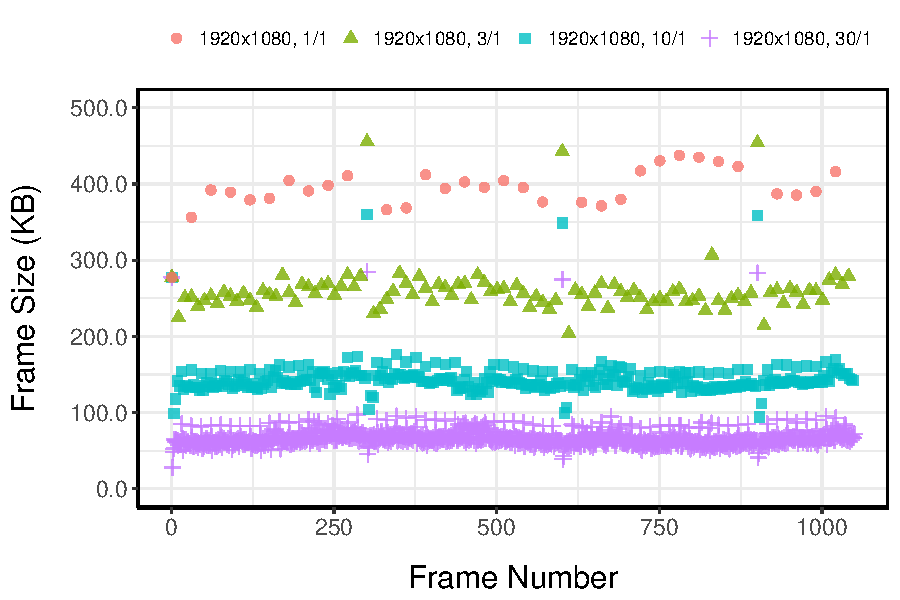
\includegraphics[width=\columnwidth]{figures/h264.pdf}
  \caption{H.264 requires more information per frame when the frame rate is
    reduced. All measurements are for videos with 1920x1080 resolution and the
    same H.264 configurations. 1/1, 3/1, 10/1 and 30/1 in the legend mean that
    the frame rates are 1 FPS, 3 FPS, 10 FPS and 30 FPS.}
  \label{fig:h264}
\end{figure}

\vspace{0.5em}

I argue that when using the above strawman solution, developers are forced to
manually study and measure the effect of individual degradation policy,
prohibiting its wide adoption in practice.

On the other extreme of the design spectrum lies a completely developer-free
solution. It is not practical, either. While static analysis has been shown to
optimize application execution adaptively in a mobile-cloud
context~\cite{chun2011clonecloud}, it only concerns with computation placement
(on the mobile or in the cloud) rather than tuning application parameters.  For
our dataflow programming model, static analysis is prone to false positives:
exploring wrong or unnecessary parameters. For example, when the application is
configured to generates statistics with a \texttt{timed\_window} operation,
static analysis may falsely detect the duration parameter and alter the behavior
of the application in an unexpected way. Also, as we will illustrate
in~\autoref{sec:profiling}, with each introduced parameter, the profiling time
increases drastically as all parameters pose a combinatorial space. The
explosion of search space prohibits explorations of unnecessary parameters.

\sysname{} takes a middle ground between these two extremes: developers use a
novel \texttt{maybe} API to annotate degradation operations without being exact
on the values. Think of these APIs as hints from developers: this operation,
when in use, will likely reduce the data size and affect the data fidelity;
however the exact quantity is not clear.

The basic form of \texttt{maybe} operator takes two arguments: a knob and a
degradation function (see \autoref{tab:operators}). The knob indicates different
degradation levels; the function performs the actual degradation operation with
a configurable level. There is one restriction on the type signature of the
function argument: $f(T, I) \Rightarrow I$. That is, the degradation function
should not alter the type of the stream. While this seems a strong restriction,
when combined with the \texttt{map} operator, the API set is still expressive
enough. I describe the implementation and usage of the APIs
in~\autoref{sec:implementation}.

Based on the \texttt{maybe} primitive, one can implement wrappers for common
degradation operations. For example, \texttt{maybe\_skip} will optionally
subsample a stream; \texttt{maybe\_downsample} can adjust the image resolution
to a configured target. Using the \texttt{maybe} API, the example mentioned
earlier can now be implemented as follows:

\begin{lstlisting}
   let app = Camera::new((1920, 1080, 30))
      .maybe_downsample(vec![(1600, 900), (1280, 720)])
      .maybe_skip(vec![2, 5])
      .map(|frame| frame.show())
      .compose();
\end{lstlisting}

This snippet first instantiates a \texttt{Camera} source, which has the type
\texttt{Stream<Image>}. It's configured to produce images with 1920x1080
resolution and 30 FPS. Two degradation operations are chained after the source:
one that downsamples the resolution to either 1600x900 or 1280x720; the other
skips frames with a parameter of 2 or 5, resulting in $30 / (2+1) = 10$ FPS or
$30/(5+1) = 5$ FPS. After the degradation, images are shown on the display; in
practice, further processing operators can be chained after the degradation.

While the API itself has simplified the specification of degradation, the exact
amount has to be known for precise rate adjustment at runtime. We then turn to
the second stage of our system that performs the automatic profiling.

\section{Multi-dimensional Profiling}
\label{sec:profiling}

The goal of this profiling stage is to explore the bandwidth-accuracy trade-off
and learn a Pareto-optimal \textit{profile} for a specific application and its
target scenario.

First, we define the terms and notations. Each \texttt{maybe} operator within an
application corresponds to a knob $k$. Suppose the application has $n$ knobs,
their combination forms a configuration $c = [k_{1}, k_{2}, ... k_{n}]$. The set
of all configurations $\mathbb{C}$ is the space that our profiling system need
to explore.

There are two mappings that we are interested: a mapping from a particular
configuration to its bandwidth requirement $B(c)$ and the accuracy measure
$A(c)$. The Pareto-optimal set $\mathbb{P}$ can then be defined
(\autoref{eq:pareto}): for all $c \in \mathbb{P}$, there is no alternative
configuration $c'$ that requires less bandwidth while giving a higher accuracy.

{\small
\begin{equation}
  \mathbb{P} = \{ c \in \mathbb{C} : \{ c' \in \mathbb{C}: B(c') < B(c),
  A(c') > A(c) \} = \varnothing\}
  \label{eq:pareto}
\end{equation}
}%

\begin{table}
  \centering
  \begin{tabular}{r l}
    \toprule
    \textbf{Symbol} & \textbf{Description} \\
    \midrule
    $n$ & number of degradation operations \\
    $k_i$ & the \textit{i}-th degradation knob \\
    $c = [k_{1}, k_{2}, ... k_{n}]$ & one specific configuration \\
    $\mathbb{C}$ & the set of all configurations \\
    \midrule
    $B(c)$ & bandwidth requirement for $c$ \\
    $A(c)$ & accuracy measure for $c$ \\
    $\mathbb{P}$ & Pareto efficienct set \\
    \bottomrule
  \end{tabular}
  \caption{Notations used in profiling.}
  \label{tab:notations}
\end{table}

Since there is often no closed form relation for $B(c)$ and $A(c)$, for
arbitrary degradation operations, \sysname{} takes a data-driven approach: with
a representative dataset and an application-specific utility function, the
system evaluates each configuration for their bandwidth demand and the
application utility. The utility could either be measured against the
groundtruth; or in the case when labelled dataset is not available, the system
uses the reference results when all degradations are turned off.

\begin{figure}
  \centering
  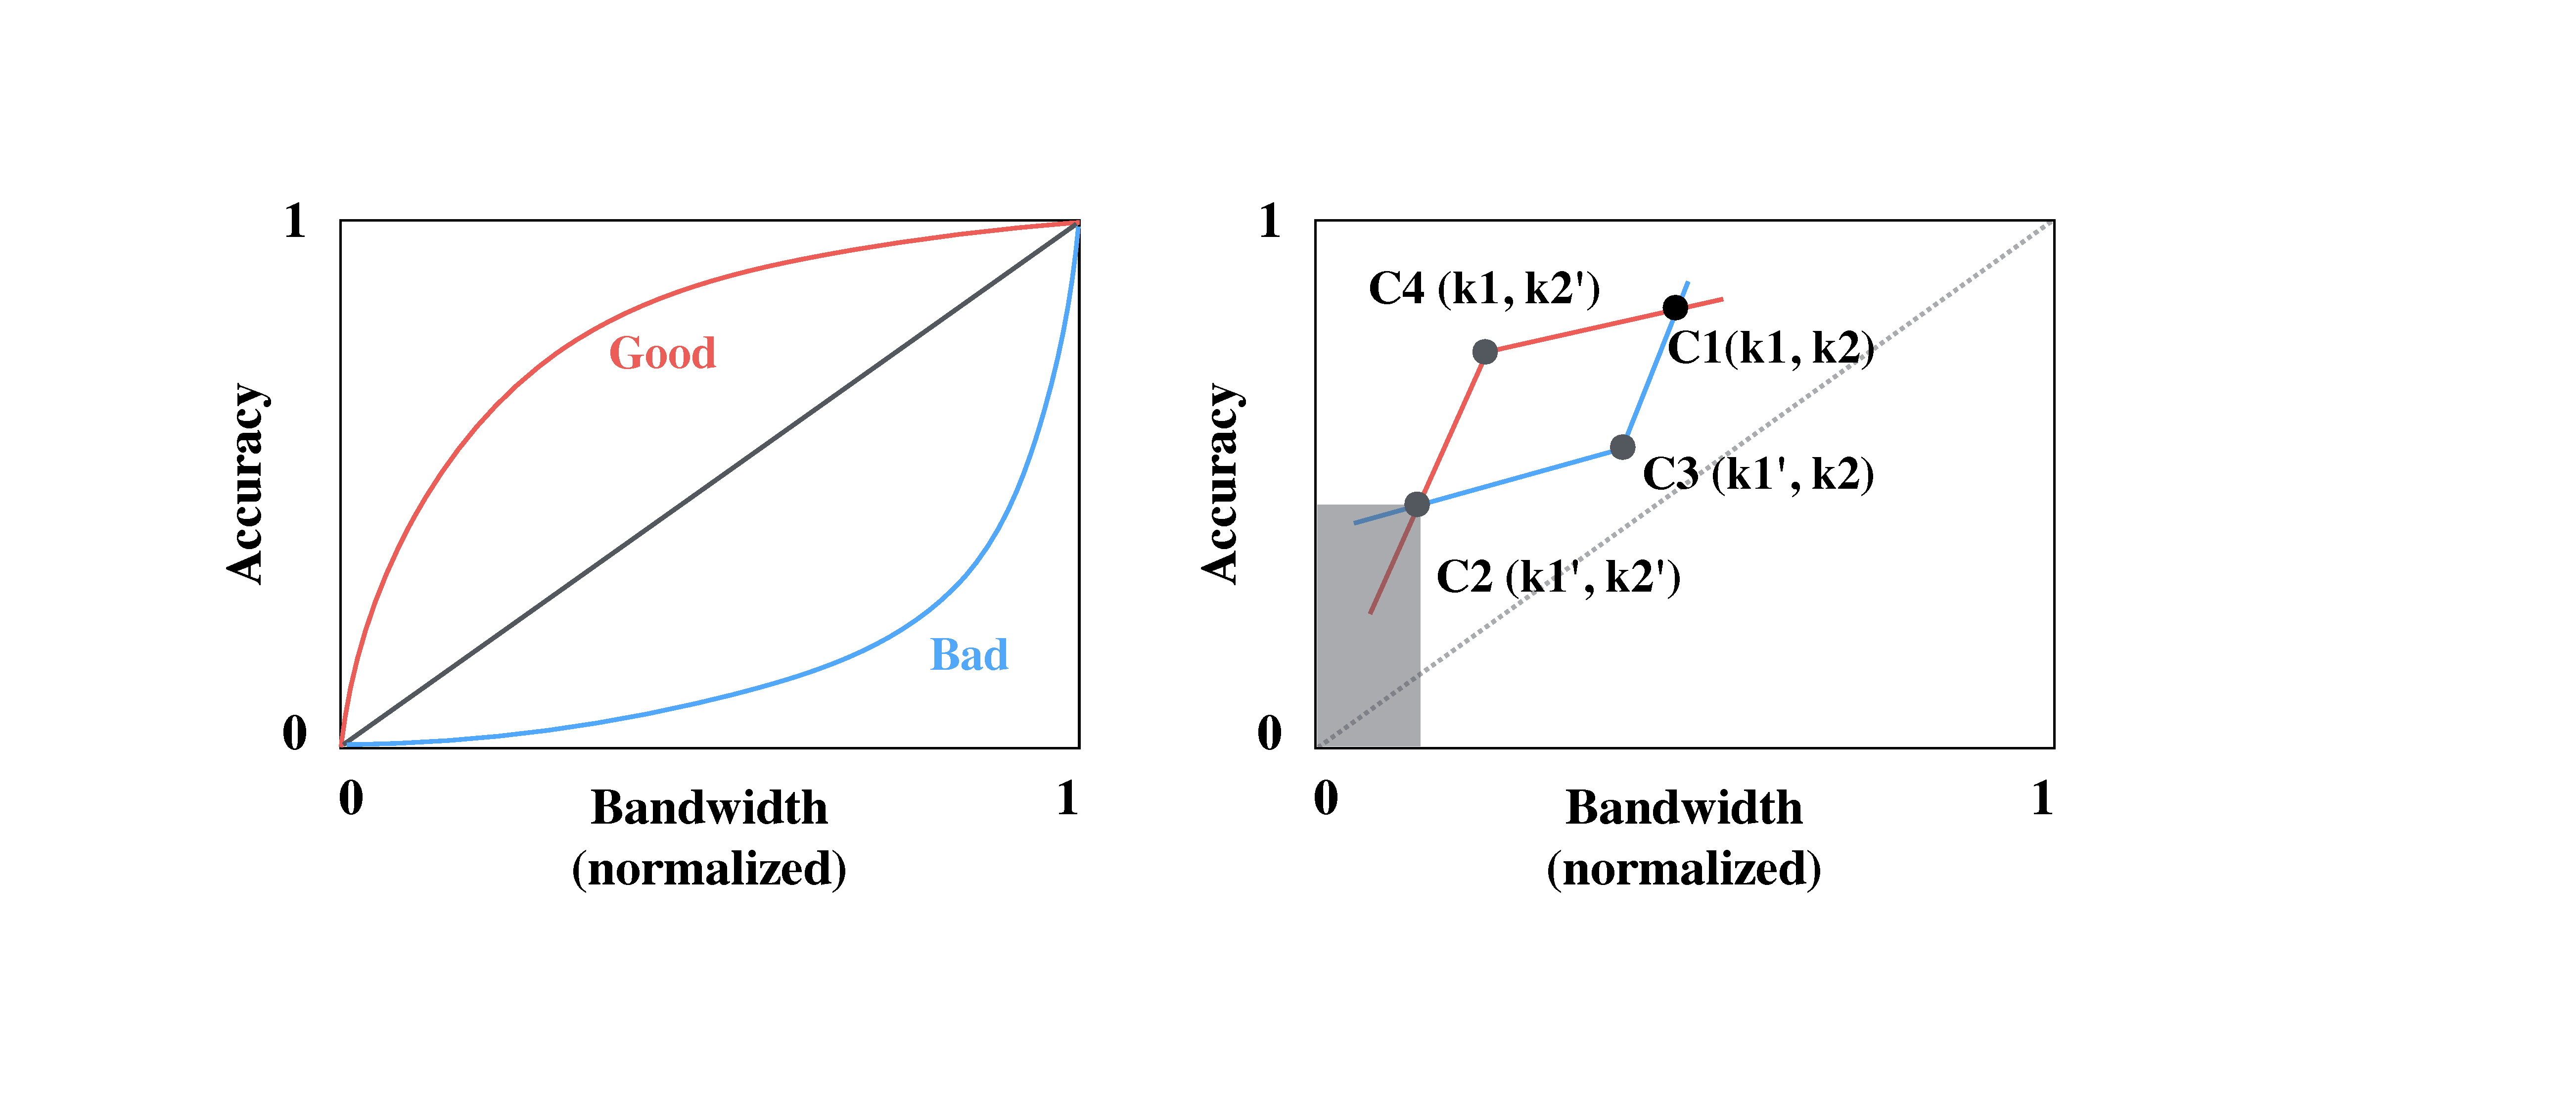
\includegraphics[width=\columnwidth]{figures/degrade.pdf}
  \caption{Illustration on the behavior of different degradation operations.}
  \label{fig:bat}
\end{figure}

When only one knob is involved, we can represent its impact using
bandwidth-accuracy curve (\autoref{fig:bat} left). The point on the curve has a
coordinate $(B(c), A(c))$ when configuration $c$ is used. The straight line from
(0, 0) to (1, 1) splits the space into two parts. Along this line, the amount of
bandwidth saving leads to an equal amount of accuracy drop (when both quantity
normalized to 1). If a degradation's profile lies above this line, it indicates
an effective degradation that should be employed as it offers little accuracy
drop with more bandwidth savings. For degradation operations below the straight
line, data information loss is more severe than the savings when the degradation
is in effect. One quantity to capture the relative power of different
degradation strategy is to use the area under the curve (AUC). With this setup,
the Pareto-optimal strategy can be define as the curve that has a maximal AUC.
We will show a few concrete profile curves in~\autoref{sec:evaluation}.

While $B(c)$ and $A(c)$ are usually monotonic along individual dimension $k_i$,
when multiple degradations combined, each curve may have a distinct shape. The
right side of \autoref{fig:bat} illustrates this complex
relationship. \todo{write more}.

Although the complexity of degradation operations prohibits further
optimizations to reduce the profiling time, there are several techniques in
practice that can make the problem tractable: (i) Exploring these configurations
is an offline task; there is no direct dependencies among configurations,
resulting in an embarrassingly parallel task. Executed in a cluster, it scales
out perfectly with provided compute resources. (ii) When the degradation level
increases or when multiple degradation operations are in effect, the amount of
data to be analyzed becomes smaller; also the computational complexity for each
data item can also be dramatically reduced. (iii) Developers can specify a lower
bound on the accuracy and the profiling can stop exploring worse configurations.
Once there is a known configuration that is worse than the configured threshold,
configurations with a larger level of degradation do not need to be profiled
(such as the gray area in \autoref{fig:bat}).

\section{Runtime Adaptation}
\label{sec:adaptation}

\begin{figure}
  \centering
  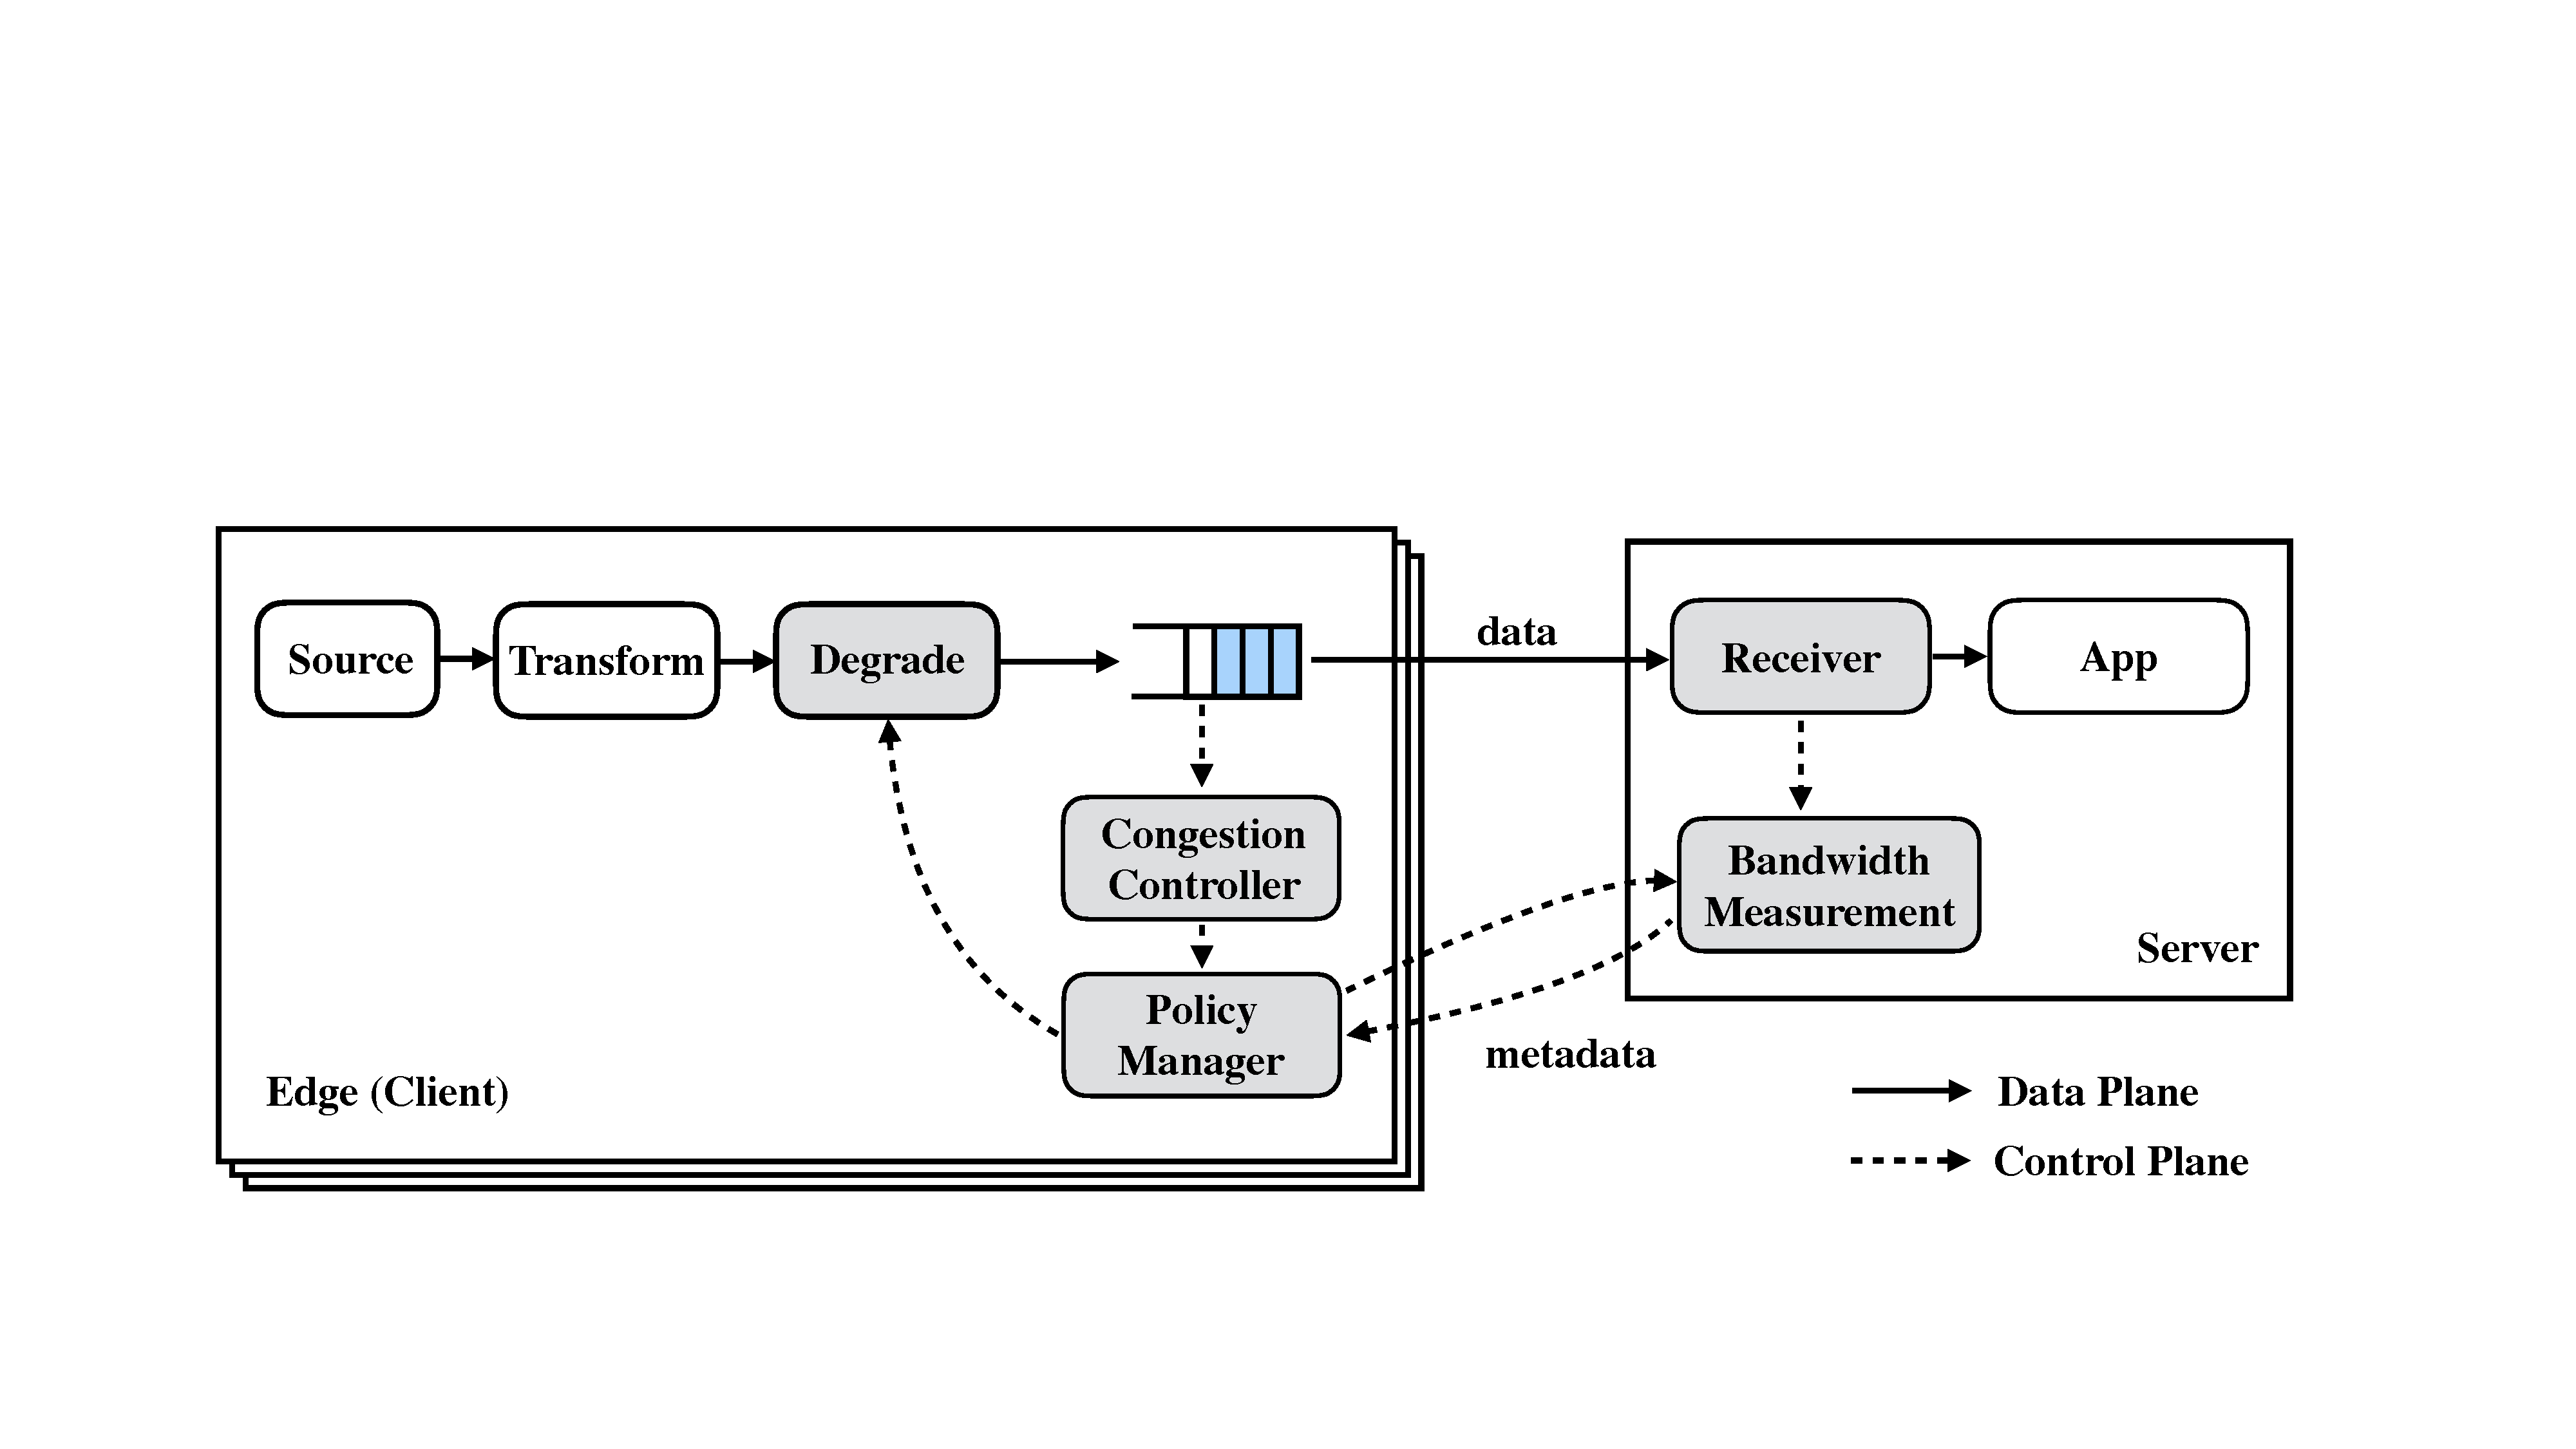
\includegraphics[width=\linewidth]{figures/runtime.pdf}
  \caption{Runtime adaptation system architecture. \sysname{}'s provided
    components are grey: they form the control plane to compensate the
    application's data plane.}
  \label{fig:runtime}
\end{figure}

\todo{stop here.} At runtime, the user program is automatically converted to a
client half and server half; and \sysname{} abstracts the communication as well
as rate adaptation. \autoref{fig:runtime} shows our runtime architecture.

\para{Object-level queue:} The queue bridges data generation and
the network capacity. It transmits data as fast as the network can handle and
detects congestion when the queue grows.

\para{Congestion controller:} Our first prototype used the queue length as a
signal for congestions, this turns out to be a bad match as the degradation
operation may change object arrival rate (e.g.\,lower frame rate for video). Our
next version uses data size, but it also leads to long latency when the
degradation changes individual object size (e.g.\,lower resolution). Our current
design uses an adaptive size: given current configuration and the profile, the
queue learns the desired data generation rate (bps), and with a user configured
latency, the queue derive the congestion watermark.

\para{Bandwidth Measurement:} The receiver delivers the received data to
application. In the meantime, it measures the effective throughput between each
client-server pair as an indication of current bandwidth~\cite{iperf}. To avoid
spikes in the bandwidth measurement, exponential smoothing is employed. While
the receiver performs bandwidth measurement every second, it does not send the
information back to each client.  avoid unnecessary communication, the client
requests the measurement only when congestion is detected.

\para{Policy Manager:} Upon receiving signals from congestion controller, it
performs an RPC request to the server for current bandwidth measurement. With
the learned profile, it determines the degradation level and start the actual
degradation strategy. The bandwidth specification in the learned profile is the
required bandwidth, the policy manager usually takes a conservative approach:
using a constant rate ALPHA to adjust the available bandwidth. When the
congestion is resolved, the policy manager gradually reduce the degradation
level (additive increase phase).

\para{Degrade:} The actual degradation operation is rather simple. Operators
based on the \texttt{maybe} API supports a \texttt{set} function that would
change the internals of the operator. The \texttt{set} function is invoked when
degradation is needed.

%% {Interaction with TCP:} Our runtime system follow the tuning guide
%% \cite{tierney2001tcp} to adjust the send buffer.

%%% Local Variables:
%%% mode: latex
%%% TeX-master: "sigcomm2017"
%%% End:

%%% Local Variables:
%%% mode: latex
%%% TeX-master: "thesis"
%%% End:
